\section{Network configuration}
The network configuration is important because each camera produces a lot of data.
The different network parameters are described in the following sections.



\subsection{Jumbo Frames}
An Ethernet frame is a unit of packetized formatted information that includes the Ethernet header, payload, and CRC trailer. \cite{winterCisco3ComApplied2009}.
The original Ethernet specification, IEEE 802.3 \cite{ieeeIEEEStandardsInterpretation2002}, allowed for a frame size between 64 to 1518 bytes, with a standard header length of 18 bytes.
Ethernet Jumbo frames carry more payload than the maximum specified by IEEE 802.3, with an \gls{mtu} size of up to 9000 bytes \cite{lucidvisionlabsJumboFramesLUCID2020}.
Increasing the maximal \gls{mtu} size typically leads to improved performance for high-bandwidth cameras and can also help reduce the CPU load on the host system \cite{lucidvisionlabsJumboFramesLUCID2020}, as there is less protocol overhead \cite{lukeThingsYouShould2018}.
Both the ethernet card used on the \jx as well as the \cams support Jumbo frames \cite{IntelI350am4Chipa} \cite{TritonMPPolarized2020a}.

\subsection{Receive Buffers}
When network packets arrive on Linux they are stored in a driver queue as shown in Figure \ref{fig:linux_network} \cite{danQueueingLinuxNetwork2013}.
The maximal number \gls{skb} can be configured using \mintinline{bash}{ethtool -G} command. \cite{danQueueingLinuxNetwork2013}.
The default and maximum number of receive buffers on the \jx are 256 and 4096, according to the \mintinline{bash}{ethtool -g eth1} command.
To avoid starvation and increase performance, it is recommended to use the use the default value to the maximal one \cite{lucidvisionlabsReceiveBuffers2020} \cite{danQueueingLinuxNetwork2013}.
As we are receiving large amounts of data as jumbo frames it is also recommended to increase the default maximal receive buffer size, which can be done permanently by running the following commands \cite{lucidvisionlabsReceiveBuffers2020}.
\begin{minted}{bash}
    $ sudo sh -c "echo 'net.core.rmem_default=1048576' >> /etc/sysctl.conf"
    $ sudo sh -c "echo 'net.core.rmem_max=1048576' >> /etc/sysctl.conf"
    $ sudo sysctl -p
\end{minted}


The receive buffer is the system memory used by the Ethernet adapter to receive packets \cite{lucidvisionlabsReceiveBuffers2020}.
Default receive buffer values set by network adapter drivers or the operating system can be low, leading to decreased performance.
The default and maximal number of receive buffers on the \jx are 256 and 4096.
This was found using the \mintinline{bash}{ethtool -g eth1} command.
It is recommended by the camera manufacturers to increase these values \cite{lucidvisionlabsReceiveBuffers2020}.
For this to have the desired effect, it is
The
\begin{figure}
    \centering
    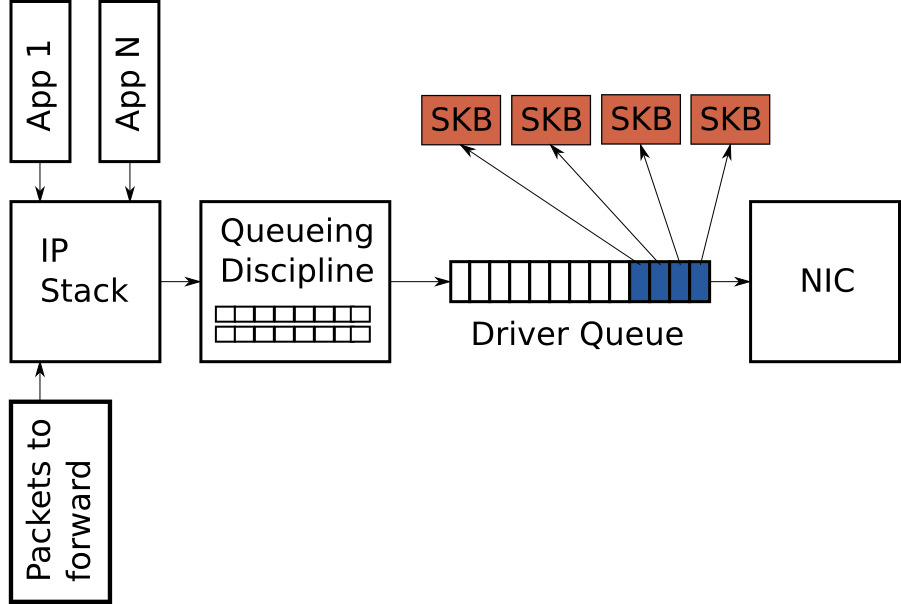
\includegraphics[width=\textwidth]{figures/linux_networking.png}
    \caption{Simplified high level overview of the queues on the transmit path of the Linux network stack \cite{danQueueingLinuxNetwork2013}}
    \label{fig:linux_network}
\end{figure}

\begin{figure*}
    \centering
    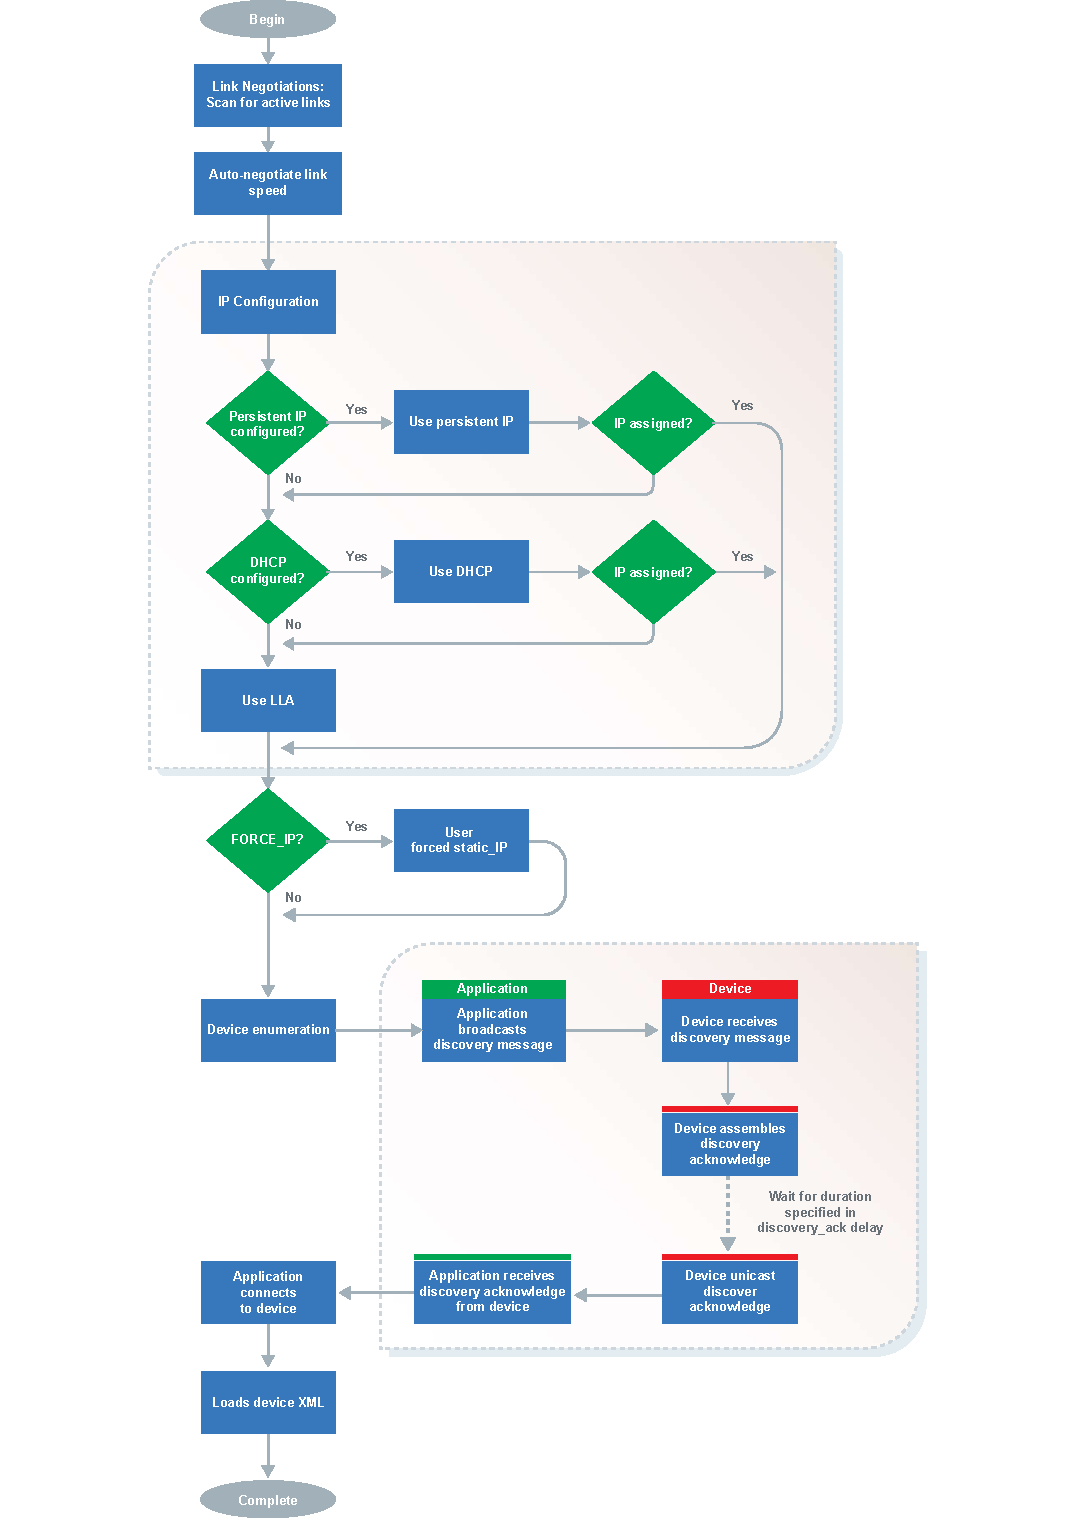
\includegraphics[width=\textwidth]{figures/thing.pdf}
    \caption{Lucid cameras are discovered and enumeration \cite{TritonMPPolarized2020}}
    \label{fig:lucid_discovery}
\end{figure*}